\documentclass[a4paper,12pt]{article}
\usepackage[margin=18mm]{geometry}
\usepackage{tikz}
\usepackage{amsmath}
\newcommand{\pFourCell}[2]{\makebox[#1em][c]{\ensuremath{#2}}}
\pagestyle{empty}
\begin{document}
\section*{Spaltentreue LaTeX-Ausgabe}
\noindent Gleichung: \texttt{sin(sqrt((x+3)/(2+1))+1)=5} \hfill Zielvariable: \texttt{x} \hfill Profil: \texttt{standard}

\vspace{8mm}
\begin{center}
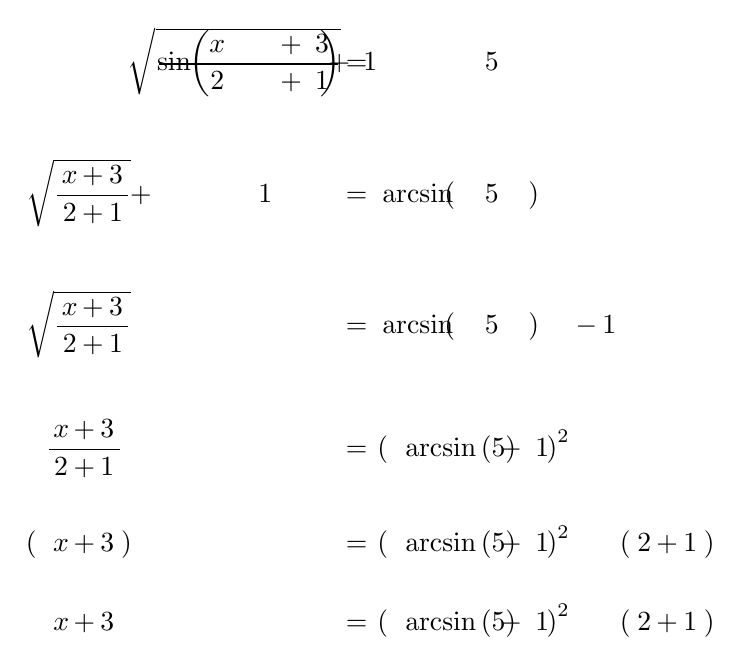
\begin{tikzpicture}[x=1em,y=-1em]
\node[anchor=base, inner sep=0pt] at (8.59,2.9) {$\pFourCell{6.46}{\sqrt{\displaystyle\frac{\pFourCell{4.22}{x}\pFourCell{1.12}{+}\pFourCell{1.12}{3}}{\pFourCell{4.22}{2}\pFourCell{1.12}{+}\pFourCell{1.12}{1}}}}\pFourCell{1.12}{+}\pFourCell{1.12}{1}$};
\node[anchor=base, inner sep=0pt] at (5.29,2.9) {$\pFourCell{1.62}{\sin}$};
\node[anchor=base, inner sep=0pt] at (6.29,2.9) {$\pFourCell{0.38}{\left(\vphantom{\pFourCell{6.46}{\sqrt{\displaystyle\frac{\pFourCell{4.22}{x}\pFourCell{1.12}{+}\pFourCell{1.12}{3}}{\pFourCell{4.22}{2}\pFourCell{1.12}{+}\pFourCell{1.12}{1}}}}\pFourCell{1.12}{+}\pFourCell{1.12}{1}}\right.}$};
\node[anchor=base, inner sep=0pt] at (10.89,2.9) {$\pFourCell{0.38}{\left.\vphantom{\pFourCell{6.46}{\sqrt{\displaystyle\frac{\pFourCell{4.22}{x}\pFourCell{1.12}{+}\pFourCell{1.12}{3}}{\pFourCell{4.22}{2}\pFourCell{1.12}{+}\pFourCell{1.12}{1}}}}\pFourCell{1.12}{+}\pFourCell{1.12}{1}}\right)}$};
\node[anchor=base, inner sep=0pt] at (11.89,2.9) {$=$};
\node[anchor=base, inner sep=0pt] at (16.77,2.9) {$5$};
\node[anchor=base, inner sep=0pt] at (1.85,7.65) {$\pFourCell{2.94}{\sqrt{\displaystyle\frac{\pFourCell{0.9}{x}\pFourCell{0.78}{+}\pFourCell{0.88}{3}}{\pFourCell{0.9}{2}\pFourCell{0.78}{+}\pFourCell{0.88}{1}}}}$};
\node[anchor=base, inner sep=0pt] at (4.09,7.65) {$+$};
\node[anchor=base, inner sep=0pt] at (8.59,7.65) {$1$};
\node[anchor=base, inner sep=0pt] at (11.89,7.65) {$=$};
\node[anchor=base, inner sep=0pt] at (16.77,7.65) {$\pFourCell{2.54}{5}$};
\node[anchor=base, inner sep=0pt] at (14.1,7.65) {$\pFourCell{2.04}{\arcsin}$};
\node[anchor=base, inner sep=0pt] at (15.31,7.65) {$\pFourCell{0.38}{\left(\vphantom{\pFourCell{2.54}{5}}\right.}$};
\node[anchor=base, inner sep=0pt] at (18.23,7.65) {$\pFourCell{0.38}{\left.\vphantom{\pFourCell{2.54}{5}}\right)}$};
\node[anchor=base, inner sep=0pt] at (1.85,12.4) {$\pFourCell{2.94}{\sqrt{\displaystyle\frac{\pFourCell{0.9}{x}\pFourCell{0.78}{+}\pFourCell{0.88}{3}}{\pFourCell{0.9}{2}\pFourCell{0.78}{+}\pFourCell{0.88}{1}}}}$};
\node[anchor=base, inner sep=0pt] at (11.89,12.4) {$=$};
\node[anchor=base, inner sep=0pt] at (16.77,12.4) {$\pFourCell{2.54}{5}$};
\node[anchor=base, inner sep=0pt] at (14.1,12.4) {$\pFourCell{2.04}{\arcsin}$};
\node[anchor=base, inner sep=0pt] at (15.31,12.4) {$\pFourCell{0.38}{\left(\vphantom{\pFourCell{2.54}{5}}\right.}$};
\node[anchor=base, inner sep=0pt] at (18.23,12.4) {$\pFourCell{0.38}{\left.\vphantom{\pFourCell{2.54}{5}}\right)}$};
\node[anchor=base, inner sep=0pt] at (20.19,12.4) {$-$};
\node[anchor=base, inner sep=0pt] at (21.02,12.4) {$1$};
\node[anchor=base, inner sep=0pt] at (2.04,16.825) {$\displaystyle\frac{\pFourCell{0.9}{x}\pFourCell{0.78}{+}\pFourCell{0.88}{3}}{\pFourCell{0.9}{2}\pFourCell{0.78}{+}\pFourCell{0.88}{1}}$};
\node[anchor=base, inner sep=0pt] at (11.89,16.825) {$=$};
\node[anchor=base, inner sep=0pt] at (16.77,16.825) {$\pFourCell{2.54}{\arcsin\left(5\right)}\pFourCell{1.12}{-}\pFourCell{1.12}{1}$};
\node[anchor=base, inner sep=0pt] at (12.89,16.825) {$\pFourCell{0.38}{\left(\vphantom{\pFourCell{2.54}{\arcsin\left(5\right)}\pFourCell{1.12}{-}\pFourCell{1.12}{1}}\right.}$};
\node[anchor=base, inner sep=0pt] at (19.11,16.825) {$\pFourCell{1.38}{\left.\vphantom{\pFourCell{2.54}{\arcsin\left(5\right)}\pFourCell{1.12}{-}\pFourCell{1.12}{1}}\right)^{2}}$};
\node[anchor=base, inner sep=0pt] at (2.04,20.285) {$\pFourCell{0.9}{x}\pFourCell{0.78}{+}\pFourCell{0.88}{3}$};
\node[anchor=base, inner sep=0pt] at (0.19,20.285) {$\pFourCell{0.38}{\left(\vphantom{\pFourCell{0.9}{x}\pFourCell{0.78}{+}\pFourCell{0.88}{3}}\right.}$};
\node[anchor=base, inner sep=0pt] at (3.51,20.285) {$\pFourCell{0.38}{\left.\vphantom{\pFourCell{0.9}{x}\pFourCell{0.78}{+}\pFourCell{0.88}{3}}\right)}$};
\node[anchor=base, inner sep=0pt] at (11.89,20.285) {$=$};
\node[anchor=base, inner sep=0pt] at (16.77,20.285) {$\pFourCell{2.54}{\arcsin\left(5\right)}\pFourCell{1.12}{-}\pFourCell{1.12}{1}$};
\node[anchor=base, inner sep=0pt] at (12.89,20.285) {$\pFourCell{0.38}{\left(\vphantom{\pFourCell{2.54}{\arcsin\left(5\right)}\pFourCell{1.12}{-}\pFourCell{1.12}{1}}\right.}$};
\node[anchor=base, inner sep=0pt] at (19.11,20.285) {$\pFourCell{1.38}{\left.\vphantom{\pFourCell{2.54}{\arcsin\left(5\right)}\pFourCell{1.12}{-}\pFourCell{1.12}{1}}\right)^{2}}$};
\node[anchor=base, inner sep=0pt] at (23.11,20.285) {$\pFourCell{0.88}{2}\pFourCell{0.78}{+}\pFourCell{0.88}{1}$};
\node[anchor=base, inner sep=0pt] at (21.65,20.285) {$\pFourCell{0.38}{\left(\vphantom{\pFourCell{0.88}{2}\pFourCell{0.78}{+}\pFourCell{0.88}{1}}\right.}$};
\node[anchor=base, inner sep=0pt] at (24.57,20.285) {$\pFourCell{0.38}{\left.\vphantom{\pFourCell{0.88}{2}\pFourCell{0.78}{+}\pFourCell{0.88}{1}}\right)}$};
\node[anchor=base, inner sep=0pt] at (1.21,23.105) {$x$};
\node[anchor=base, inner sep=0pt] at (2.05,23.105) {$+$};
\node[anchor=base, inner sep=0pt] at (2.88,23.105) {$3$};
\node[anchor=base, inner sep=0pt] at (11.89,23.105) {$=$};
\node[anchor=base, inner sep=0pt] at (16.77,23.105) {$\pFourCell{2.54}{\arcsin\left(5\right)}\pFourCell{1.12}{-}\pFourCell{1.12}{1}$};
\node[anchor=base, inner sep=0pt] at (12.89,23.105) {$\pFourCell{0.38}{\left(\vphantom{\pFourCell{2.54}{\arcsin\left(5\right)}\pFourCell{1.12}{-}\pFourCell{1.12}{1}}\right.}$};
\node[anchor=base, inner sep=0pt] at (19.11,23.105) {$\pFourCell{1.38}{\left.\vphantom{\pFourCell{2.54}{\arcsin\left(5\right)}\pFourCell{1.12}{-}\pFourCell{1.12}{1}}\right)^{2}}$};
\node[anchor=base, inner sep=0pt] at (23.11,23.105) {$\pFourCell{0.88}{2}\pFourCell{0.78}{+}\pFourCell{0.88}{1}$};
\node[anchor=base, inner sep=0pt] at (21.65,23.105) {$\pFourCell{0.38}{\left(\vphantom{\pFourCell{0.88}{2}\pFourCell{0.78}{+}\pFourCell{0.88}{1}}\right.}$};
\node[anchor=base, inner sep=0pt] at (24.57,23.105) {$\pFourCell{0.38}{\left.\vphantom{\pFourCell{0.88}{2}\pFourCell{0.78}{+}\pFourCell{0.88}{1}}\right)}$};
\end{tikzpicture}
\end{center}

\newpage
\section*{Spaltentreue LaTeX-Ausgabe mit Spaltengrenzen}
\vspace{6mm}
\begin{center}
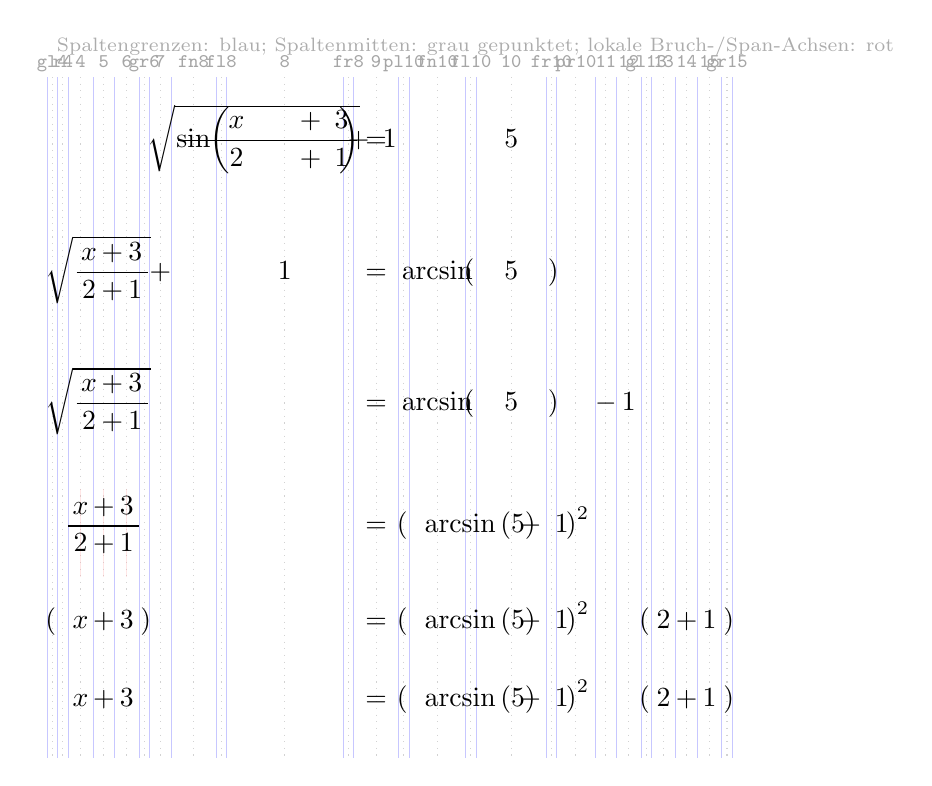
\begin{tikzpicture}[x=1em,y=-1em]
\node[font={\scriptsize}, text=gray!65, anchor=west] at (0,-0.75) {Spaltengrenzen: blau; Spaltenmitten: grau gepunktet; lokale Bruch-/Span-Achsen: rot};
\draw[blue!22, line width=0.28pt] (0,0.35) -- (0,24.94);
\draw[blue!22, line width=0.28pt] (0.38,0.35) -- (0.38,24.94);
\draw[blue!22, line width=0.28pt] (0.76,0.35) -- (0.76,24.94);
\draw[blue!22, line width=0.28pt] (1.66,0.35) -- (1.66,24.94);
\draw[blue!22, line width=0.28pt] (2.44,0.35) -- (2.44,24.94);
\draw[blue!22, line width=0.28pt] (3.32,0.35) -- (3.32,24.94);
\draw[blue!22, line width=0.28pt] (3.7,0.35) -- (3.7,24.94);
\draw[blue!22, line width=0.28pt] (4.48,0.35) -- (4.48,24.94);
\draw[blue!22, line width=0.28pt] (6.1,0.35) -- (6.1,24.94);
\draw[blue!22, line width=0.28pt] (6.48,0.35) -- (6.48,24.94);
\draw[blue!22, line width=0.28pt] (10.7,0.35) -- (10.7,24.94);
\draw[blue!22, line width=0.28pt] (11.08,0.35) -- (11.08,24.94);
\draw[blue!22, line width=0.28pt] (12.7,0.35) -- (12.7,24.94);
\draw[blue!22, line width=0.28pt] (13.08,0.35) -- (13.08,24.94);
\draw[blue!22, line width=0.28pt] (15.12,0.35) -- (15.12,24.94);
\draw[blue!22, line width=0.28pt] (15.5,0.35) -- (15.5,24.94);
\draw[blue!22, line width=0.28pt] (18.04,0.35) -- (18.04,24.94);
\draw[blue!22, line width=0.28pt] (18.42,0.35) -- (18.42,24.94);
\draw[blue!22, line width=0.28pt] (19.8,0.35) -- (19.8,24.94);
\draw[blue!22, line width=0.28pt] (20.58,0.35) -- (20.58,24.94);
\draw[blue!22, line width=0.28pt] (21.46,0.35) -- (21.46,24.94);
\draw[blue!22, line width=0.28pt] (21.84,0.35) -- (21.84,24.94);
\draw[blue!22, line width=0.28pt] (22.72,0.35) -- (22.72,24.94);
\draw[blue!22, line width=0.28pt] (23.5,0.35) -- (23.5,24.94);
\draw[blue!22, line width=0.28pt] (24.38,0.35) -- (24.38,24.94);
\draw[blue!22, line width=0.28pt] (24.76,0.35) -- (24.76,24.94);
\draw[gray!35, dotted] (0.19,0.35) -- (0.19,24.94);
\node[font={\ttfamily\scriptsize}, text=gray!70, anchor=base] at (0.19,0) {gl4};
\draw[gray!35, dotted] (0.57,0.35) -- (0.57,24.94);
\node[font={\ttfamily\scriptsize}, text=gray!70, anchor=base] at (0.57,0) {r4};
\draw[gray!35, dotted] (1.21,0.35) -- (1.21,24.94);
\node[font={\ttfamily\scriptsize}, text=gray!70, anchor=base] at (1.21,0) {4};
\draw[gray!35, dotted] (2.05,0.35) -- (2.05,24.94);
\node[font={\ttfamily\scriptsize}, text=gray!70, anchor=base] at (2.05,0) {5};
\draw[gray!35, dotted] (2.88,0.35) -- (2.88,24.94);
\node[font={\ttfamily\scriptsize}, text=gray!70, anchor=base] at (2.88,0) {6};
\draw[gray!35, dotted] (3.51,0.35) -- (3.51,24.94);
\node[font={\ttfamily\scriptsize}, text=gray!70, anchor=base] at (3.51,0) {gr6};
\draw[gray!35, dotted] (4.09,0.35) -- (4.09,24.94);
\node[font={\ttfamily\scriptsize}, text=gray!70, anchor=base] at (4.09,0) {7};
\draw[gray!35, dotted] (5.29,0.35) -- (5.29,24.94);
\node[font={\ttfamily\scriptsize}, text=gray!70, anchor=base] at (5.29,0) {fn8};
\draw[gray!35, dotted] (6.29,0.35) -- (6.29,24.94);
\node[font={\ttfamily\scriptsize}, text=gray!70, anchor=base] at (6.29,0) {fl8};
\draw[gray!35, dotted] (8.59,0.35) -- (8.59,24.94);
\node[font={\ttfamily\scriptsize}, text=gray!70, anchor=base] at (8.59,0) {8};
\draw[gray!35, dotted] (10.89,0.35) -- (10.89,24.94);
\node[font={\ttfamily\scriptsize}, text=gray!70, anchor=base] at (10.89,0) {fr8};
\draw[gray!35, dotted] (11.89,0.35) -- (11.89,24.94);
\node[font={\ttfamily\scriptsize}, text=gray!70, anchor=base] at (11.89,0) {9};
\draw[gray!35, dotted] (12.89,0.35) -- (12.89,24.94);
\node[font={\ttfamily\scriptsize}, text=gray!70, anchor=base] at (12.89,0) {pl10};
\draw[gray!35, dotted] (14.1,0.35) -- (14.1,24.94);
\node[font={\ttfamily\scriptsize}, text=gray!70, anchor=base] at (14.1,0) {fn10};
\draw[gray!35, dotted] (15.31,0.35) -- (15.31,24.94);
\node[font={\ttfamily\scriptsize}, text=gray!70, anchor=base] at (15.31,0) {fl10};
\draw[gray!35, dotted] (16.77,0.35) -- (16.77,24.94);
\node[font={\ttfamily\scriptsize}, text=gray!70, anchor=base] at (16.77,0) {10};
\draw[gray!35, dotted] (18.23,0.35) -- (18.23,24.94);
\node[font={\ttfamily\scriptsize}, text=gray!70, anchor=base] at (18.23,0) {fr10};
\draw[gray!35, dotted] (19.11,0.35) -- (19.11,24.94);
\node[font={\ttfamily\scriptsize}, text=gray!70, anchor=base] at (19.11,0) {pr10};
\draw[gray!35, dotted] (20.19,0.35) -- (20.19,24.94);
\node[font={\ttfamily\scriptsize}, text=gray!70, anchor=base] at (20.19,0) {11};
\draw[gray!35, dotted] (21.02,0.35) -- (21.02,24.94);
\node[font={\ttfamily\scriptsize}, text=gray!70, anchor=base] at (21.02,0) {12};
\draw[gray!35, dotted] (21.65,0.35) -- (21.65,24.94);
\node[font={\ttfamily\scriptsize}, text=gray!70, anchor=base] at (21.65,0) {gl13};
\draw[gray!35, dotted] (22.28,0.35) -- (22.28,24.94);
\node[font={\ttfamily\scriptsize}, text=gray!70, anchor=base] at (22.28,0) {13};
\draw[gray!35, dotted] (23.11,0.35) -- (23.11,24.94);
\node[font={\ttfamily\scriptsize}, text=gray!70, anchor=base] at (23.11,0) {14};
\draw[gray!35, dotted] (23.94,0.35) -- (23.94,24.94);
\node[font={\ttfamily\scriptsize}, text=gray!70, anchor=base] at (23.94,0) {15};
\draw[gray!35, dotted] (24.57,0.35) -- (24.57,24.94);
\node[font={\ttfamily\scriptsize}, text=gray!70, anchor=base] at (24.57,0) {gr15};
\node[anchor=base, inner sep=0pt] at (8.59,2.9) {$\pFourCell{6.46}{\sqrt{\displaystyle\frac{\pFourCell{4.22}{x}\pFourCell{1.12}{+}\pFourCell{1.12}{3}}{\pFourCell{4.22}{2}\pFourCell{1.12}{+}\pFourCell{1.12}{1}}}}\pFourCell{1.12}{+}\pFourCell{1.12}{1}$};
\node[anchor=base, inner sep=0pt] at (5.29,2.9) {$\pFourCell{1.62}{\sin}$};
\node[anchor=base, inner sep=0pt] at (6.29,2.9) {$\pFourCell{0.38}{\left(\vphantom{\pFourCell{6.46}{\sqrt{\displaystyle\frac{\pFourCell{4.22}{x}\pFourCell{1.12}{+}\pFourCell{1.12}{3}}{\pFourCell{4.22}{2}\pFourCell{1.12}{+}\pFourCell{1.12}{1}}}}\pFourCell{1.12}{+}\pFourCell{1.12}{1}}\right.}$};
\node[anchor=base, inner sep=0pt] at (10.89,2.9) {$\pFourCell{0.38}{\left.\vphantom{\pFourCell{6.46}{\sqrt{\displaystyle\frac{\pFourCell{4.22}{x}\pFourCell{1.12}{+}\pFourCell{1.12}{3}}{\pFourCell{4.22}{2}\pFourCell{1.12}{+}\pFourCell{1.12}{1}}}}\pFourCell{1.12}{+}\pFourCell{1.12}{1}}\right)}$};
\node[anchor=base, inner sep=0pt] at (11.89,2.9) {$=$};
\node[anchor=base, inner sep=0pt] at (16.77,2.9) {$5$};
\node[anchor=base, inner sep=0pt] at (1.85,7.65) {$\pFourCell{2.94}{\sqrt{\displaystyle\frac{\pFourCell{0.9}{x}\pFourCell{0.78}{+}\pFourCell{0.88}{3}}{\pFourCell{0.9}{2}\pFourCell{0.78}{+}\pFourCell{0.88}{1}}}}$};
\node[anchor=base, inner sep=0pt] at (4.09,7.65) {$+$};
\node[anchor=base, inner sep=0pt] at (8.59,7.65) {$1$};
\node[anchor=base, inner sep=0pt] at (11.89,7.65) {$=$};
\node[anchor=base, inner sep=0pt] at (16.77,7.65) {$\pFourCell{2.54}{5}$};
\node[anchor=base, inner sep=0pt] at (14.1,7.65) {$\pFourCell{2.04}{\arcsin}$};
\node[anchor=base, inner sep=0pt] at (15.31,7.65) {$\pFourCell{0.38}{\left(\vphantom{\pFourCell{2.54}{5}}\right.}$};
\node[anchor=base, inner sep=0pt] at (18.23,7.65) {$\pFourCell{0.38}{\left.\vphantom{\pFourCell{2.54}{5}}\right)}$};
\node[anchor=base, inner sep=0pt] at (1.85,12.4) {$\pFourCell{2.94}{\sqrt{\displaystyle\frac{\pFourCell{0.9}{x}\pFourCell{0.78}{+}\pFourCell{0.88}{3}}{\pFourCell{0.9}{2}\pFourCell{0.78}{+}\pFourCell{0.88}{1}}}}$};
\node[anchor=base, inner sep=0pt] at (11.89,12.4) {$=$};
\node[anchor=base, inner sep=0pt] at (16.77,12.4) {$\pFourCell{2.54}{5}$};
\node[anchor=base, inner sep=0pt] at (14.1,12.4) {$\pFourCell{2.04}{\arcsin}$};
\node[anchor=base, inner sep=0pt] at (15.31,12.4) {$\pFourCell{0.38}{\left(\vphantom{\pFourCell{2.54}{5}}\right.}$};
\node[anchor=base, inner sep=0pt] at (18.23,12.4) {$\pFourCell{0.38}{\left.\vphantom{\pFourCell{2.54}{5}}\right)}$};
\node[anchor=base, inner sep=0pt] at (20.19,12.4) {$-$};
\node[anchor=base, inner sep=0pt] at (21.02,12.4) {$1$};
\draw[red!30, opacity=0.32, line width=0.35pt] (1.21,15.25) -- (1.21,18.4);
\draw[red!30, opacity=0.32, line width=0.35pt] (2.05,15.25) -- (2.05,18.4);
\draw[red!30, opacity=0.32, line width=0.35pt] (2.88,15.25) -- (2.88,18.4);
\node[anchor=base, inner sep=0pt] at (2.04,16.825) {$\displaystyle\frac{\pFourCell{0.9}{x}\pFourCell{0.78}{+}\pFourCell{0.88}{3}}{\pFourCell{0.9}{2}\pFourCell{0.78}{+}\pFourCell{0.88}{1}}$};
\node[anchor=base, inner sep=0pt] at (11.89,16.825) {$=$};
\node[anchor=base, inner sep=0pt] at (16.77,16.825) {$\pFourCell{2.54}{\arcsin\left(5\right)}\pFourCell{1.12}{-}\pFourCell{1.12}{1}$};
\node[anchor=base, inner sep=0pt] at (12.89,16.825) {$\pFourCell{0.38}{\left(\vphantom{\pFourCell{2.54}{\arcsin\left(5\right)}\pFourCell{1.12}{-}\pFourCell{1.12}{1}}\right.}$};
\node[anchor=base, inner sep=0pt] at (19.11,16.825) {$\pFourCell{1.38}{\left.\vphantom{\pFourCell{2.54}{\arcsin\left(5\right)}\pFourCell{1.12}{-}\pFourCell{1.12}{1}}\right)^{2}}$};
\node[anchor=base, inner sep=0pt] at (2.04,20.285) {$\pFourCell{0.9}{x}\pFourCell{0.78}{+}\pFourCell{0.88}{3}$};
\node[anchor=base, inner sep=0pt] at (0.19,20.285) {$\pFourCell{0.38}{\left(\vphantom{\pFourCell{0.9}{x}\pFourCell{0.78}{+}\pFourCell{0.88}{3}}\right.}$};
\node[anchor=base, inner sep=0pt] at (3.51,20.285) {$\pFourCell{0.38}{\left.\vphantom{\pFourCell{0.9}{x}\pFourCell{0.78}{+}\pFourCell{0.88}{3}}\right)}$};
\node[anchor=base, inner sep=0pt] at (11.89,20.285) {$=$};
\node[anchor=base, inner sep=0pt] at (16.77,20.285) {$\pFourCell{2.54}{\arcsin\left(5\right)}\pFourCell{1.12}{-}\pFourCell{1.12}{1}$};
\node[anchor=base, inner sep=0pt] at (12.89,20.285) {$\pFourCell{0.38}{\left(\vphantom{\pFourCell{2.54}{\arcsin\left(5\right)}\pFourCell{1.12}{-}\pFourCell{1.12}{1}}\right.}$};
\node[anchor=base, inner sep=0pt] at (19.11,20.285) {$\pFourCell{1.38}{\left.\vphantom{\pFourCell{2.54}{\arcsin\left(5\right)}\pFourCell{1.12}{-}\pFourCell{1.12}{1}}\right)^{2}}$};
\node[anchor=base, inner sep=0pt] at (23.11,20.285) {$\pFourCell{0.88}{2}\pFourCell{0.78}{+}\pFourCell{0.88}{1}$};
\node[anchor=base, inner sep=0pt] at (21.65,20.285) {$\pFourCell{0.38}{\left(\vphantom{\pFourCell{0.88}{2}\pFourCell{0.78}{+}\pFourCell{0.88}{1}}\right.}$};
\node[anchor=base, inner sep=0pt] at (24.57,20.285) {$\pFourCell{0.38}{\left.\vphantom{\pFourCell{0.88}{2}\pFourCell{0.78}{+}\pFourCell{0.88}{1}}\right)}$};
\node[anchor=base, inner sep=0pt] at (1.21,23.105) {$x$};
\node[anchor=base, inner sep=0pt] at (2.05,23.105) {$+$};
\node[anchor=base, inner sep=0pt] at (2.88,23.105) {$3$};
\node[anchor=base, inner sep=0pt] at (11.89,23.105) {$=$};
\node[anchor=base, inner sep=0pt] at (16.77,23.105) {$\pFourCell{2.54}{\arcsin\left(5\right)}\pFourCell{1.12}{-}\pFourCell{1.12}{1}$};
\node[anchor=base, inner sep=0pt] at (12.89,23.105) {$\pFourCell{0.38}{\left(\vphantom{\pFourCell{2.54}{\arcsin\left(5\right)}\pFourCell{1.12}{-}\pFourCell{1.12}{1}}\right.}$};
\node[anchor=base, inner sep=0pt] at (19.11,23.105) {$\pFourCell{1.38}{\left.\vphantom{\pFourCell{2.54}{\arcsin\left(5\right)}\pFourCell{1.12}{-}\pFourCell{1.12}{1}}\right)^{2}}$};
\node[anchor=base, inner sep=0pt] at (23.11,23.105) {$\pFourCell{0.88}{2}\pFourCell{0.78}{+}\pFourCell{0.88}{1}$};
\node[anchor=base, inner sep=0pt] at (21.65,23.105) {$\pFourCell{0.38}{\left(\vphantom{\pFourCell{0.88}{2}\pFourCell{0.78}{+}\pFourCell{0.88}{1}}\right.}$};
\node[anchor=base, inner sep=0pt] at (24.57,23.105) {$\pFourCell{0.38}{\left.\vphantom{\pFourCell{0.88}{2}\pFourCell{0.78}{+}\pFourCell{0.88}{1}}\right)}$};
\end{tikzpicture}
\end{center}
\end{document}
